\documentclass{article}
\usepackage{microtype,graphicx,booktabs,hyperref,amsmath,amssymb}
\newcommand{\theHalgorithm}{\arabic{algorithm}}
\usepackage[preprint]{icml2026}
\icmltitlerunning{Coupled Physical-Event Contracts: An Audited Component Study}
\makeatletter\gdef\icmlcorrespondingauthor@text{Author details pending}\makeatother
\begin{document}
\twocolumn[
\icmltitle{Coupled Physical-Event Contracts for Robot Experience:\\Task-Graph Expansion and an Audited Component Study}
\begin{icmlauthorlist}\icmlauthor{Research development draft}{draft}\end{icmlauthorlist}
\icmlaffiliation{draft}{Component report; shared-policy and chemical evaluation remain open}
\vskip .3in]
\printAffiliationsAndNotice{}
\begin{abstract}
Laboratory operations constrain physical effects, not merely command dispatch.
Dependencies, persistent processes and original event references can make
apparently timely actions violate the task. We develop independently scored
event contracts and examine two components. An exact scheduling candidate
matches exhaustive enumeration on 7,172 synthetic interval conditions; the
preserved earlier planner incorrectly rejects 61 feasible conditions. A separate
MuJoCo experiment executes 12 controlled trajectories across four task graphs,
plus two separately reported sentinels. A reference-preserving graph controller
satisfies all four registered contracts, compared with one for an unguarded
graph controller and none for an independent-window ordering baseline.
These fixed mechanical cases validate interfaces and expose failure modes.
They do not establish learned-policy improvement, chemical outcomes, real-time
agent execution or generalization. The proposed learning study must absorb
verified recovery experience under matched budgets and independent evaluation.
\end{abstract}

\section{Problem and motivation}
Consider stopping addition within two seconds after an endpoint appears, or
maintaining actual stirring for a prescribed duration while another operation
shares the robot. The deadline applies to an effective event such as stopped
flow or motion. A prompt command can still produce a late physical effect;
restarting a process can create a timely-looking result while abandoning the
original experiment. We propose studying experience generation, verification
and absorption under these original physical contracts.

The benchmark's C5, C6 and C13 definitions remain unchanged. C5 requests a
two-second endpoint-to-stop response; C6 specifies 120$\pm$10 seconds of actual
stirring; C13 includes a transient A cue and randomized A-to-B waiting in a
no-clock track. The current twin-rotor fixture is separately registered and
does not certify any of these chemical tasks. Preserved A-r7 robot timing
evidence also remains separate: one fixed instance and three earlier trials.

\paragraph{Positioning.}
Physical-time representations are already studied by Chronos
\cite{chronos}, while remaining-time control, punctuality, recovery and
coordination are considered by \citet{timecontrol}. Agent context and robot
self-improvement are studied by GPT-Policy and RoboRSI
\cite{gptpolicy,roborsi}. Thus adding time to DP or assembling an agent training
pipeline is insufficient as a novelty claim. Our proposed emphasis is the
interaction of independently measured event contracts, immutable original
references, concurrent process preservation and verified experience absorption.
The component evidence below supports infrastructure development, not the
full proposed contribution.

\section{Physical-event formulation}
Let a task contain an event dependency graph $G$, contracts $\Phi$, observation
rules $O$ and resource capacities $R$. Observation capture and delivery,
command dispatch and physical effect have distinct timestamps. The actor
uses only permitted delivered observations, public task information and past
legal history. An independent scorer uses raw physical measurements, which
are not passed back as privileged actor inputs.

An event occurrence is a conservative interval $I_e=[\ell_e,u_e]$ on one
identified physical clock. Confirmation time is retained separately. For an
event-to-event target $D$ and tolerance $\epsilon$, score
\[ I_{\rm error}=[\ell_b-u_a-D,\;u_b-\ell_a-D]. \]
TRUE requires containment in $[-\epsilon,\epsilon]$; disjointness is FALSE;
overlap without containment is UNKNOWN. Missing and left-censored events
cannot count as success. Formal joint success conjoins timing, required
physical predicates, dependency, original-reference and safety conditions.
Strict sampled maintenance is reported explicitly; it does not establish
continuity between physical samples.

For the proposed general system, the reference ledger retains already established original anchors. Recovery
cannot relabel a reference or reset a process and count it as the same task.
An infeasible original contract remains failed or safely stopped; a restarted
process is a new task instance. Cold reconstruction does not establish
continuous process time without an independent continuous clock and evolution.

\section{Joint scheduling component}
For a public cue $c$, desired contact after $D$, contact-to-release gap $H$,
known FIFO delay $\delta$ and mechanical latency boxes
$a\in[a_L,a_U]$, $b\in[b_L,b_U]$, feasible grid dispatches satisfy
{\small\begin{align*}
d_A-c&\in[D-\epsilon-\delta-a_L,\ D+\epsilon-\delta-a_U],\\
d_B-c&\in[D+H-\epsilon-\delta-b_L,\ D+H+\epsilon-\delta-b_U],\\
d_B-d_A&\in[H-\epsilon-b_L+a_U,\ H+\epsilon-b_U+a_L].
\end{align*}}
The preserved skill also imposes a minimum stage gap and an earliest contact
dispatch. The same constant FIFO delay for both events cancels from the gap but not from the
absolute windows. Two separate absolute-window passes permit opposing errors
and therefore do not imply the gap contract.

The candidate uses exact rational constraints. For each feasible contact grid
tick, intersect the release grid bounds with the gap and minimum-skill bounds.
The objective minimizes squared distance to midpoint dispatches, with
deterministic grid tie-breaking. For fixed contact, the convex release term
attains its discrete minimum at a clamped floor/ceiling of the ideal release;
checking these points suffices. Independently enumerated all-pair constraints
and a third integer implementation check the returned feasibility and choice.
This is classical finite scheduling, not a new general safety theorem.
Soundness applies only to the supplied box, resource and skill assumptions;
an empirical calibration envelope is not true uncertainty support.

The source and roster were frozen before the full matrix. It contains 6,912
factorial conditions, 256 fixed-seed synthetic draws and four targeted
boundaries. Grid periods, latency widths, delay, tolerances and skill minimums
vary. Every exception and refusal remains in the 7,172-condition denominator.
Synthetic draws are not physical random seeds or robot episodes.

\begin{table}[t]\centering\small
\caption{Synthetic interval conditions. Denominator 7,172 in every row;
2,606 conditions are mathematically feasible. No physical episode credit.}
\begin{tabular}{lrr}\toprule
Method & Robust joint & Exceptions\\\midrule
Nominal prior & 409 & 975 \\
Public delay & 788 & 981 \\
Independent midpoint & 2375 & 1198 \\
Old joint & 2545 & 1198 \\
Exact candidate & 2606 & 0 \\
\bottomrule\end{tabular}\end{table}

The candidate matches complete enumeration in every condition, including
4,566 infeasible cases. Independent enumeration checks 299,040 grid pairs.
The old joint planner falsely refuses 61 feasible cases, because it rejects
a negative independent-midpoint release hold before its joint search.
Its scheduled outputs have no erroneous robust acceptance in this matrix.
The independent midpoint schedules also have 994 cases in which both
absolute event windows pass while their gap fails. The candidate remains
separate from the preserved native A source; the latter is not silently fixed.

\section{Task-graph physics component}
A preserved contact-free twin-rotor MJCF is integrated by MuJoCo at 10 ms.
Four registered graphs are parallel, A-before-B, B-before-A and A-while-B-active.
A shared serial command bus and a global relay have measured effective
control schedules. All three controllers receive the same delivered state,
public graph, service model and fixed calibration set. Private true dynamics,
reference truth and scorer labels are withheld. Dynamics and fault setting
are fixed inside the calibration set; this is a development component with
no multi-seed or learned task-space generalization claim.

The ordering baseline retains an A-before-B command form and checks
independent endpoint windows. The graph scheduler searches graph-constrained
command forms and can use the global relay. The guarded variant additionally
protects predicted original reference acquisition. These are hand-written
controllers, not learned policies or a reproduction of an earlier history agent.

Each of 12 main trajectories and two sentinels integrates one complete ten-second
epoch: 14,014 controlled state samples. One independently reconstructed
full-power trajectory supplies counterfactual benchmark reference crossing intervals
(1,001 diagnostic samples); 100 preflight steps are counted separately.
This fixture compares actual crossings with that fixed counterfactual bracket.
It does not validate a ledger recovery for an externally observed, already
occurred chemical event.
No task-period state/time write or reset occurs. Stops require a previously
moving rotor followed by at least 200 ms of low-speed samples: 21 points,
with onset brackets distinct from confirmation. B preservation conjoins
sampled torque and motion predicates until its required original bound.
The independent audit re-integrates all controls and recomputes all contracts.

\begin{table}[t]\centering\small
\caption{Main mechanical contracts: four instances per controller. The
two sentinels are excluded from this table and reported separately.}
\begin{tabular}{lrrr}\toprule
Controller & TRUE & FALSE & UNKNOWN\\\midrule
Independent windows & 0 & 4 & 0 \\
Graph constraints & 1 & 3 & 0 \\
Graph + reference guard & 4 & 0 & 0 \\
\bottomrule\end{tabular}\end{table}

The feasible sentinel satisfies its original contract. The dependency-cycle
sentinel correctly produces no commands, integrates its full trace, and remains
FALSE in physical contract scoring; correct refusal is separately recorded.
All twelve main cases remain in their original denominator; both sentinels
are reported separately.
The controlled dispatch/delivery delays advance native time, but host planning
work pauses this fixture. Consequently these results do not establish physical
continuity during real model waits or wall-clock timing guarantees.

\begin{figure}[t]\centering
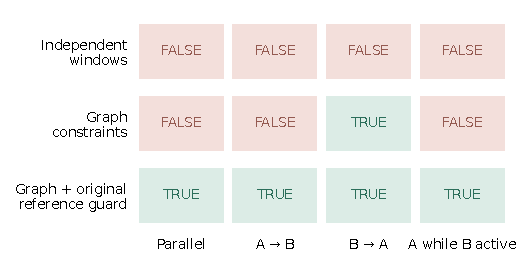
\includegraphics[width=\columnwidth]{figures/task_graph_contracts_compact.pdf}
\caption{Independent original-contract verdicts for the four registered
graphs. Fixed mechanical cases; hand-written rules; no new weights.}
\end{figure}

\section{Proposed learning study and open gates}
The agent should compile tasks, choose data, diagnose failures and propose
recoveries. A fast executor preserves physical processes; the independent
verifier determines data admission. Verified successes, failures and valid
recoveries retain original anchors in replay. The initial learning study
compares shared DP inputs under one backbone: no added time, legal public
time, capture/execution timestamps and past history with reset/shuffle controls.

Teacher relabeling on student-visited states must match teacher identity,
labels, optimization, native steps and compute to offline imitation. If the
update is supervised aggregation, it is DAgger-style \cite{dagger}; a distinct
on-policy distillation objective must be specified before claiming OPD.
Offline and online RL are conditional ablations, rather than mandatory stages.
Context reset tests parameter absorption; frozen weights with retained history
test context adaptation. Evaluation splits full instances, not frames, and
separates state, time, graph and process-drift holdouts.

The frozen A-r7 extension plans four calibration and 16 tests, varying bottle
mass/inertia, actual position-target FIFO and joint contact/release contracts.
It has no admitted new test result in this component report. After initial
resource refusal, its first calibration starts when one GPU satisfies the
frozen 24 GiB admission. We neither lower that bound nor preempt foreign jobs. The four-calibration
empirical envelope must pass independent raw audit before test use.

Remaining scientific gates include calibrated flow/motor/thermal endpoints,
continuous process evolution during real planner waits, independently clocked
hardware, actual shared policy weights and matched-budget held-out improvements.
The present component tests expose infrastructure errors and make the proposed
study reviewable; they do not complete the full method-paper claim.

\begin{thebibliography}{9}
\bibitem[Chronos(2026)]{chronos} Chronos Policy: Learning Robot Policies on Physical Time. 2026. \url{https://arxiv.org/abs/2610.13929}.
\bibitem[Time Control(2026)]{timecontrol} Time as a Control Dimension in Robot Learning. Version 2, 2026. \url{https://arxiv.org/abs/2511.07654}.
\bibitem[GPT-Policy(2026)]{gptpolicy} GPT-Policy. 2026. \url{https://arxiv.org/abs/2609.19138}.
\bibitem[RoboRSI(2026)]{roborsi} RoboRSI. 2026. \url{https://arxiv.org/abs/2610.12424}.
\bibitem[Ross et~al.(2011)]{dagger} Ross, S., Gordon, G., and Bagnell, D. A Reduction of Imitation Learning and Structured Prediction to No-Regret Online Learning. AISTATS, 2011. \url{https://proceedings.mlr.press/v15/ross11a.html}.
\end{thebibliography}
\end{document}
